\documentclass[12pt,a4paper,twoside,openright]{report}
	\usepackage[pdfborder={0 0 0}]{hyperref}    % turns references into hyperlinks
	\usepackage[margin=25mm]{geometry}  % adjusts page layout
	\usepackage{graphicx}  % allows inclusion of PDF, PNG and JPG images
	\usepackage{verbatim}
	\usepackage{docmute}   % only needed to allow inclusion of proposal.tex
	\usepackage{import} %import proposal from another folder
	\usepackage{pdfpages}
	\usepackage{listings}
	\usepackage{upquote}

	\raggedbottom                           % try to avoid widows and orphans
	\sloppy
	\clubpenalty1000%
	\widowpenalty1000%
	
	\renewcommand{\baselinestretch}{1.1}    % adjust line spacing to make
																					% more readable
	
	\begin{document}
	
	\bibliographystyle{plain}
	
	
	%%%%%%%%%%%%%%%%%%%%%%%%%%%%%%%%%%%%%%%%%%%%%%%%%%%%%%%%%%%%%%%%%%%%%%%%
	% Title
	
	
	\pagestyle{empty}
	
	\rightline{\LARGE \textbf{Charlie Crisp}}
	
	\vspace*{60mm}
	\begin{center}
	\Huge
	\textbf{Building a Blockchain Library for OCaml} \\[5mm]
	Computer Science Tripos -- Part II \\[5mm]
	Pembroke College \\[5mm]
	\today  % today's date
	\end{center}
	
	%%%%%%%%%%%%%%%%%%%%%%%%%%%%%%%%%%%%%%%%%%%%%%%%%%%%%%%%%%%%%%%%%%%%%%%%%%%%%%
	% Proforma, table of contents and list of figures
	
	\pagestyle{plain}
	
	\chapter*{Proforma}
	
	{\large
	\begin{tabular}{ll}
	Name:               & \bf Charlie Crisp                       \\
	College:            & \bf Pembroke College                     \\
	Project Title:      & \bf Building a Blockchain Library for OCaml \\
	Examination:        & \bf Computer Science Tripos -- Part II, July 2018  \\
	Word Count:         & \bf ????\footnotemark[1]\\
	Project Originator: & KC Sivaramakrishnan                    \\
	Supervisor:         & KC Sivaramakrishnan                    \\ 
	\end{tabular}
	}
	\stepcounter{footnote}
	
	
	\section*{Original Aims of the Project}
	
	To build a library in OCaml, which can be used as a building block for Blockchain applications. 
	The library should allow participating nodes to own a shared copy of a Blockchain data structure, agreed upon using consensus.
	Nodes should also be able to commit transactions to the blockchain, which should then be visible to other participating nodes. 
	
	
	\section*{Work Completed}
	
	All that has been completed appears in this dissertation.
	
	\section*{Special Difficulties}
	
	None
	 
	\newpage
	\section*{Declaration}
	
	I, Charlie Crisp of Pembroke College, being a candidate for Part II of the Computer
	Science Tripos, hereby declare that this dissertation and the work described in it are my own work,
	unaided except as may be specified below, and that the dissertation
	does not contain material that has already been used to any substantial
	extent for a comparable purpose.
	
	\bigskip
	\leftline{Signed}
	\bigskip
	\leftline{Date}
	
	\tableofcontents
	
	\listoffigures
	
	\newpage
	\section*{Acknowledgements}
	
	I would like to thank KC Sivaramakrishnan for being an extremely helpful supervisor throughout the duration of the dissertation, as well as over the past three years.\\
	I would also like to thank Anil Madhavapeddy for allowing me to use his laptop for the duration of the dissertation, and being a very supportive DoS.\\
	Finally I'd like to thank my friends and family for supporting me through my final year.
	
	%%%%%%%%%%%%%%%%%%%%%%%%%%%%%%%%%%%%%%%%%%%%%%%%%%%%%%%%%%%%%%%%%%%%%%%
	% now for the chapters
	
	\pagestyle{headings}
	
	\chapter{Introduction}
	Blockchain technology has existed for a long time, but the definition of 'blockchain' has changed drastically since its conception.
	Previously used just to describe a data structure, the term 'blockchain' is now widely used to also describe the accompanying consensus mechanisms.
	This is mainly due to the increasing popularity of cryptocurrencies such as Bitcoin \cite{Bitcoin} which use the 'Proof of Work' algorithm to solve the double spending problem \cite{}.
	However, whilst blockchain is undoubtably the most important technology in the field of cryptocurrencies, where no single client can be trusted, it also has many uses outside this application.
	It can be used in other situations where clients can be trusted, for instance, a hospital maintaining medical records, or a bank wishing to record transactions from many of its own distributed clients.\\
	

	I have implemented a blockchain library in OCaml which allows the easy creation of blockchain applications.
	The blockchain is synchronised via a leader-based consensus mechanism with eventual consistency.
	Because the application is written in OCaml, it can be compiled to bytecode, unikernels or even javascript and is therefore suitable for a wide range of destination applications and devices.

	\section{The History of the Blockchain}
	The blockchain, in its simplest form, is a series of blocks of data, where each block contains the cryptographic hash of the previous block in the chain. 
	Figure \ref{fig:mainblockchain} is a graphical representation of a typical blockchain data structure.
	\begin{figure}
		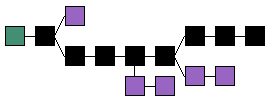
\includegraphics[width=\linewidth]{figs/blockchain}
		\caption{A typical blockchain structure}
		\label{fig:mainblockchain}
	\end{figure}
	The blockchain, as a cryptographically secure chain of blocks, was first conceptualised by Stuart Haber and W. Scott Stornetta in 1990 \cite{HaberStornetta}.
	However, until the creation of Git \cite{Git} in 2005, the blockchain was still a relatively niche concept.
	The invention of Bitcoin in 2008 is seen by many as the most pivotal moment in the history of blockchain technologies.
	Bitcoin uses the Proof of Work consensus algorithm to create a decentralised, trust-less, peer to peer network which is used to make transactions between virtual wallets.

	\section{Blockchain Today}
	At the time of writing, cryptocurrencies are generating both a huge amount of excitement and cynicism in popular media. 
	Cryptocurrencies aside from Bitcoin are paving the way to smarter uses of the blockchain.
	For example, Ethereum \cite{Ethereum} introduces the concept of Smart Contracts which allow the execution of code on the blockchain.\\
	
	Whilst it is possible to think of applications for blockchain technology in almost every sector, the development of applications outside the scope of crytocurrencies has been limited. 
	If one considers the example of OCaml, there are currently no libraries which allow a user to easily get started with building blockchain applications. \\

	\section{Work Completed}
	I have created a library which allows developers to create blockchain applications with the ease of importing a library.
	The project was designed to exist outside the realm of cryptocurrencies and therefore assumes that all participating nodes are trustworthy.
	Consensus is achieved by using a simple leader-based model where the leader node will periodically pull updates from all participating nodes and merge them into a central blockchain.
	This can then be viewed by all participating nodes, with the guarantee of eventual consistency.
	Setting up a network is as easy as specifying the location of the leader on all the participating nodes, and specifying the location of all participating nodes on the leader.\\
	
	I have evaluated the project by... FILL IN EVALUATION DETAILS

	\chapter{Preparation}
	\section{Starting Point}
		The project built upon functionality provided by Irmin [1] which is a distributed database system.  Irmin is fast, durable and has the branching capabilities which are required to build a blockchain.\\
		The project also made use of Ezirmin \cite{Ezirmin} which provides a simplified API to Irmin.\\
	\section{Using OCaml}
		At the start of the project, I had never used OCaml for any project of significance. 
		Whilst the first year Foundations of Computer Science course had given me some background into functional programming, there were still many key OCaml features which I had to learn.
		In the first few weeks of my project, I spent time studying the book Real World OCaml \cite{RealWorldOCaml} which proved a great introduction to many of OCaml's features.  
		\subsection*{Pattern Matching}
		OCaml provides a very powerful syntax for matching patterns which allow you to write functions like the following\ldots 
		\begin{lstlisting}[language=Caml,showstringspaces=false] 
  type card = Card of string * int
  let pattern_matcher_1 input = match input with 
    | Card("spades", 1) -> Printf.printf "It's the ace of spades!"
    | _ -> Printf.printf "Unlucky"
  
  let pattern_matcher_2 = function 
    | Card(class, 1) -> Printf.printf "It's the ace of %s! class"
    | _ -> Printf.printf "Unlucky"
		\end{lstlisting}
		In the first example above, we have a function that will print a special string if it is passed the Ace of Spades. 
		Here, the pattern matching checks the that the tuple associated with the data type contains the string \texttt{spades} and the number 1.\\
		The second example uses the anonymous \texttt{function} keyword and matches the first argument of the tuple to the variable \texttt{class}.
		\subsection*{Optionals}
		A built in data type that allows us to use the power of OCaml's pattern matching, is the \texttt{option}. By using the \texttt{Some(\ldots)} and \texttt{None} constructors, one can create something of the type \texttt{'a option}. \\
		\\
		This is comparable to the \texttt{null} type in languages such as Java, however as it is part of the type system, it forces the programmer to handle any cases where \texttt{null} could be returned.
		\subsection*{Error Handling}
		OCaml provides multiple different ways of dealing with errors and exceptions. 
		A simple way of signifying an error in your return type, is to return an \texttt{option} which will be \texttt{None} if there is an error. 
		Whilst this can be inflexible for larger solutions, it also provides a quick and simple way of signifying that something has gone wrong.\\
		\\
		Another way of dealing with options in return types is to use the \texttt{bind} function. This also has the infix operator $>>=$
		\begin{lstlisting}[language=Caml,showstringspaces=false]
  val bind: 'a option -> ('a -> 'b option) -> 'b option = <fun>
		\end{lstlisting} 
		As the above type signiture demonstrates, \texttt{bind} will take an \texttt{option} and apply a function to its contents if it exists, or return \texttt{None} otherwise.\\
		\\
		OCaml provides a built in type \texttt{Result.t} which is effectively an extention of optional return types, where the programmer is able to define arbitrary data to accompany the error type. The following code demonstrates a successful return type of \texttt{int} (with an unspecified \texttt{Error} type), and a \texttt{string} error type (with an unspecified \texttt{Ok} type).
		\begin{lstlisting}[language=Caml,showstringspaces=false]
  # Ok 3;;
  - : ('a, int) result = Ok 3
  # Error "Something went wrong";;
  - : (string, 'a) result = Error "Something went wrong";;
		\end{lstlisting} 
		\subsection*{Polymorphic Variants}
		OCaml allows the programmer to define variant types such as the \texttt{Card} type that was defined earlier. This makes it very easy to make use of pattern matching with custom defined types.\\
		\\
		OCaml also introduces the notion of polymorphic variants which are more flexible and do not require an explicit type declaration.
		\begin{lstlisting}[language=Caml,showstringspaces=false]
  # let card = `Card ("spades", 1);;
  - : val card : [> `Card of string * int ] = `Card ("spades", 1)
		\end{lstlisting}
		Here, we have used a backtick to define a polymorphic type, and OCaml has automatically inferred a type for us. 
		The $>$ symbol acts as a lower limit on the tags that the variant \texttt{card} can take, i.e. it can have the tag \`\texttt{Card} or indeed other unspecified tags.\\
		When dealing with variant types as parameters, we may see the $<$ symbol in the type signature to denote that the paramater can only belong to given set of tags. The absence of both of these symbols indicates that a variant has exactly the given type signature. 
		\subsection*{Development Environment}
		When developing a large scale system with OCaml, there are a couple of build systems available to use. 'jbuilder' \cite{jbuilder} is one of these systems which is becoming increasingly popular and is used daily by hundreds of developers.\\
		\\
		jbuilder allows the developer to specify arbitrary directory structures containing executables, libraries and more. Whilst setting up my project, I defined a structure consisting of three main directories: one containing the executable for running a leader node, one containing the executable for running a participant node, and one for containing utility libraries used by my project.\\
		I also used GNU Make \cite{GNUMake} to invoke jbuilder which allowed me to easily build and run any executables from the root of the directory.\\
		\\
		In order to ensure that the project would always build, I set up a continuous integration workflow using Travis-CI. 
		This was particularly useful as it ensured that whenever I pushed any updates to my GitHub repository, Travis would attempt to build the system and would notify me whenever there were any errors during the build.
	\section{Requirements Analysis}
	During the preparation stage of my project, I spent some time analysing the requirements that would be suitable for my projects. This proved a good way of guiding the progress of the project and making sure that I solved all the problems that I set out to. Here, I will set out the criteria that I decided upon before starting development on the project.
	\subsection*{Data Structure}
	A key component of this project was to build a blockchain data structure that would allow transactions to be added to a ledger. 
	From a participating node, it should be possible to add a transaction, of a given type, between two identities. 
	It should also be possible to view an ordered list of all transactions which currently exist in the blockchain.
	\subsection*{Consensus}
	Many uses of blockchain rely on achieving consensus using a Proof of Work principle. 
	Whilst this may or may not be a suitable method of achieving consensus for this project, it is important that the implementation guarantees a strict ordering of transactions in the ledger.
	I.e. should one node read a sequence of transactions from a blockchain, then all other nodes will percieve the sequence of transactions in the same order.\\
	\\
	It is also important that this consensus mechanism is scalable, and within the scope of this project, it should be possible for the blockchain to be shared by 4 or more nodes in a network. This should not hinder the performance of the system, and it should still be able to handle multiple successful transactions per second.\\
	\\
	In the case of failure for any singular node, the system should be able to recover or continue within a countable number of seconds. It would be desirable (although not a criteria for this project) for the system to be able to recover after the failure of multiple nodes, and even in the case of a network partition. 
	\chapter{Implementation}
	\section{The Blockchain Data Structure}
	\subsection*{Git as a blockchain}
		Git provides a data structure which can be interacted with via a command line API. However, it is not trivial why these data structure is classed as a blockchain. \\
		\\
		In order to convince oneself of this, it is worth considering what features are required for a data structure to be considered a blockchain. 
		Whilst there is no universally agreed definition of a blockchain, it is commonly accepted that it will exhibit the following features:
		\begin{enumerate}
			\item Data is stored in 'blocks'.
			\item Blocks are ordered.
			\item Each block contains a link to its parent block.
		\end{enumerate}
		Now we can consider the promises that Git makes and ensure that the above conditions are satisfied.\\
		\begin{enumerate}
			\item Git stores data as sequences of 'commits' which can be thought of as blocks.
			\item Git history is stored as a tree structure with arbitrary branching. This imposes an order on commits or blocks.
			\item Each Git commit contains the hash of the previous or parent commit.
		\end{enumerate}
		It is clear to see that Git has all the necessary properties to be used as a blockchain data structure.
	\subsection*{Irmin}
		The next question that I needed to answer, was how it was best to interact with an underlying Git protocol, using OCaml. Irmin is a library for OCaml which provides Git-like, distributed, branchable storage \cite{Irmin}.\\
		\\
		Irmin uses a Git backend to store objects which immediately makes it suitable for use as a blockchain. However, it is also possible to consider Irmin's data store at a higher level. \\
		\\
		Irmin provides access to a Block Store and a Tag Store as shown in figure \ref{fig:IrminBlockStore}.
		\begin{figure}
			\begin{center}
			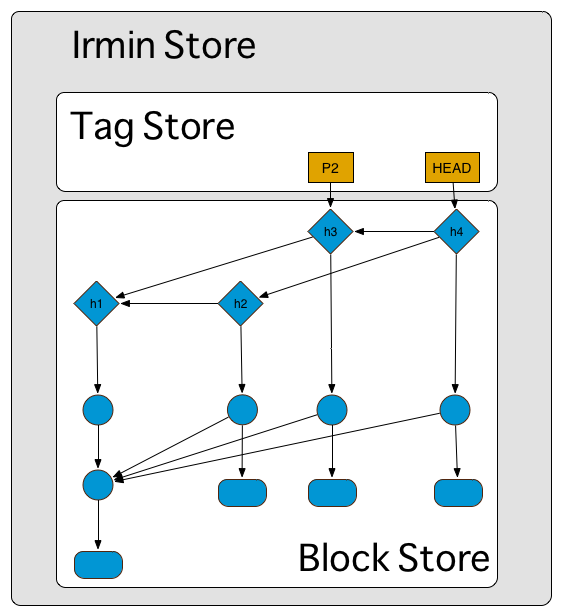
\includegraphics[width=8cm]{figs/irmin-stores.png}
			\caption{An Irmin Store composed of a mutable Tag Store and an immutable Block Store}
			\label{fig:IrminBlockStore}
			\end{center}
		\end{figure}
		The block store is an append-only store of immutable key-value pairs. Mutability comes from the tag store, which provides a way of mapping global branch names to blocks. Both of these stores combine to form an Irmin store with  promises which are beneficial for concurrency. For example, if a tag is not mutated, then you can be sure that the no change in the block store will be visible.\\
		\\
		Irmin Stores can be though of in terms of the following API, expressed in OCaml code. Here, we expose types for keys which address values, and tags which point to keys. The read and update functions allow us to interact with the block store. \\
		\begin{lstlisting}[language=Caml]
  type t
  (* The type for Irmin store. *)

  type tag
  type key 
  type value

  val read: t -> ?branch:tag -> key -> value option
  val update: t -> ?branch:tag -> key -> value -> unit
			
		\end{lstlisting}
		Amongst other different interfaces, Irmin provides a built in API for interacting with an append-only store. This key functionality of this module is expressed in the following code, where \texttt{mem} checks for the presence of a key, \texttt{find} reads values, and \texttt{add} writes to the store.

		\begin{lstlisting}[language=Caml]
  val mem: t -> key -> bool Lwt.t
  val find: t -> key -> value option Lwt.t
  val add: t -> value -> key Lwt.t
		\end{lstlisting}
	\subsection*{Ezirmin}
	Ezirmin is a library that provides a simplified interface to the Irmin library. It is designed to provide a interface to Irmin without functors, but with some useful defaults. Importantly, it has a built in log data structure which uses Irmin's append-only store, saved on disk in the git format.\\
	For this reason, I decided that it would be a suitable data structure to use in this project.
	\section{Mempools}
	When making a transaction using Bitcoin or some other cryptocurrencies, a request for this transaction is placed in what is known as a Mempool\footnote{Mempool is short for Memory Pool}.
	This Mempool can be thought of as a waiting room for transactions. When miners are assembling and mining blocks, this is where they will pick the transactions from.
	
	\section{Consensus Algorithms}
	%TODO: Explain how this was an important part of work.
	%TODO: Explain what are the problems with all of these consensus algorithms and why would they not work in my case.
	%TODO: Explain what the algorithm that I developed is and why it solves these problems
	Typically, cryptocurrencies (which rely on blockchain technology) use a Proof of Work protocol to achieve consensus. 
	There are, however, other ways of achieving consensus, and I evaluated a number of these in order to inform my approach to building consensus into my project. \\ 
		\subsection*{Existing Algorithms}
			\subsubsection*{Proof of Work}
			%TODO: This is good for solving double spending
			%TODO: How does it work in Bitcoin
			%TODO: Use a diagram, mention nonces, yada yada yada
			The proof of work method for achieving consensus is actually very simple. 
			Whenever a block is received by a participating node, the node will check that the block contains a proof of computational work done. 
			In the field of cryptocurrencies, this proof takes the form of a random sequence of data which, when appended to the end of the block, causes its hash to be prefixed with a set number of 0s.
			Because the data appended to the end of a block can only be found by a brute force method, which will require lots of computation/work.
			\subsubsection*{Proof of Stake}
			%TODO: Flesh this out with small amount of detail
			%TODO: Not good for this projects as you need the concept of Stake
			\subsubsection*{Paxos}
			%TODO: Finish
			\subsubsection*{Raft}
			%TODO: Finish description of Raft and it's concept of terms.
		\subsection*{A New Approach}
		%TODO: Overview of my approach to consensus
			\subsection*{Pros and Cons of a Leader Based Approach}
			%TODO: Why is this beneficial? It loosens the trust that comes with a leader based approach.
			%TODO: Might also increase overhead?
			%TODO: Can we do it in a low cost way?
			\subsection*{Writing to the blockchain}
			%TODO: Describe how a participant writes into a mempool that the leader then copies. Participants can then pull from it. 
			\subsection*{How to deal with failure}
			%TODO: If it's a participant then fine. Even if leader changes, that will still be part of the old leaders blockchain.
			%TODO: If it's a leader, then other participants start a leader election.

	\chapter{Evaluation}
	
	\chapter{Conclusion}
	
	
	%%%%%%%%%%%%%%%%%%%%%%%%%%%%%%%%%%%%%%%%%%%%%%%%%%%%%%%%%%%%%%%%%%%%%
	% the bibliography
	\bibliographystyle{plain}
	\bibliography{refs}
	\addcontentsline{toc}{chapter}{Bibliography}
	
	%%%%%%%%%%%%%%%%%%%%%%%%%%%%%%%%%%%%%%%%%%%%%%%%%%%%%%%%%%%%%%%%%%%%%
	% the appendices
	\appendix

	\chapter{Project Proposal}
	
	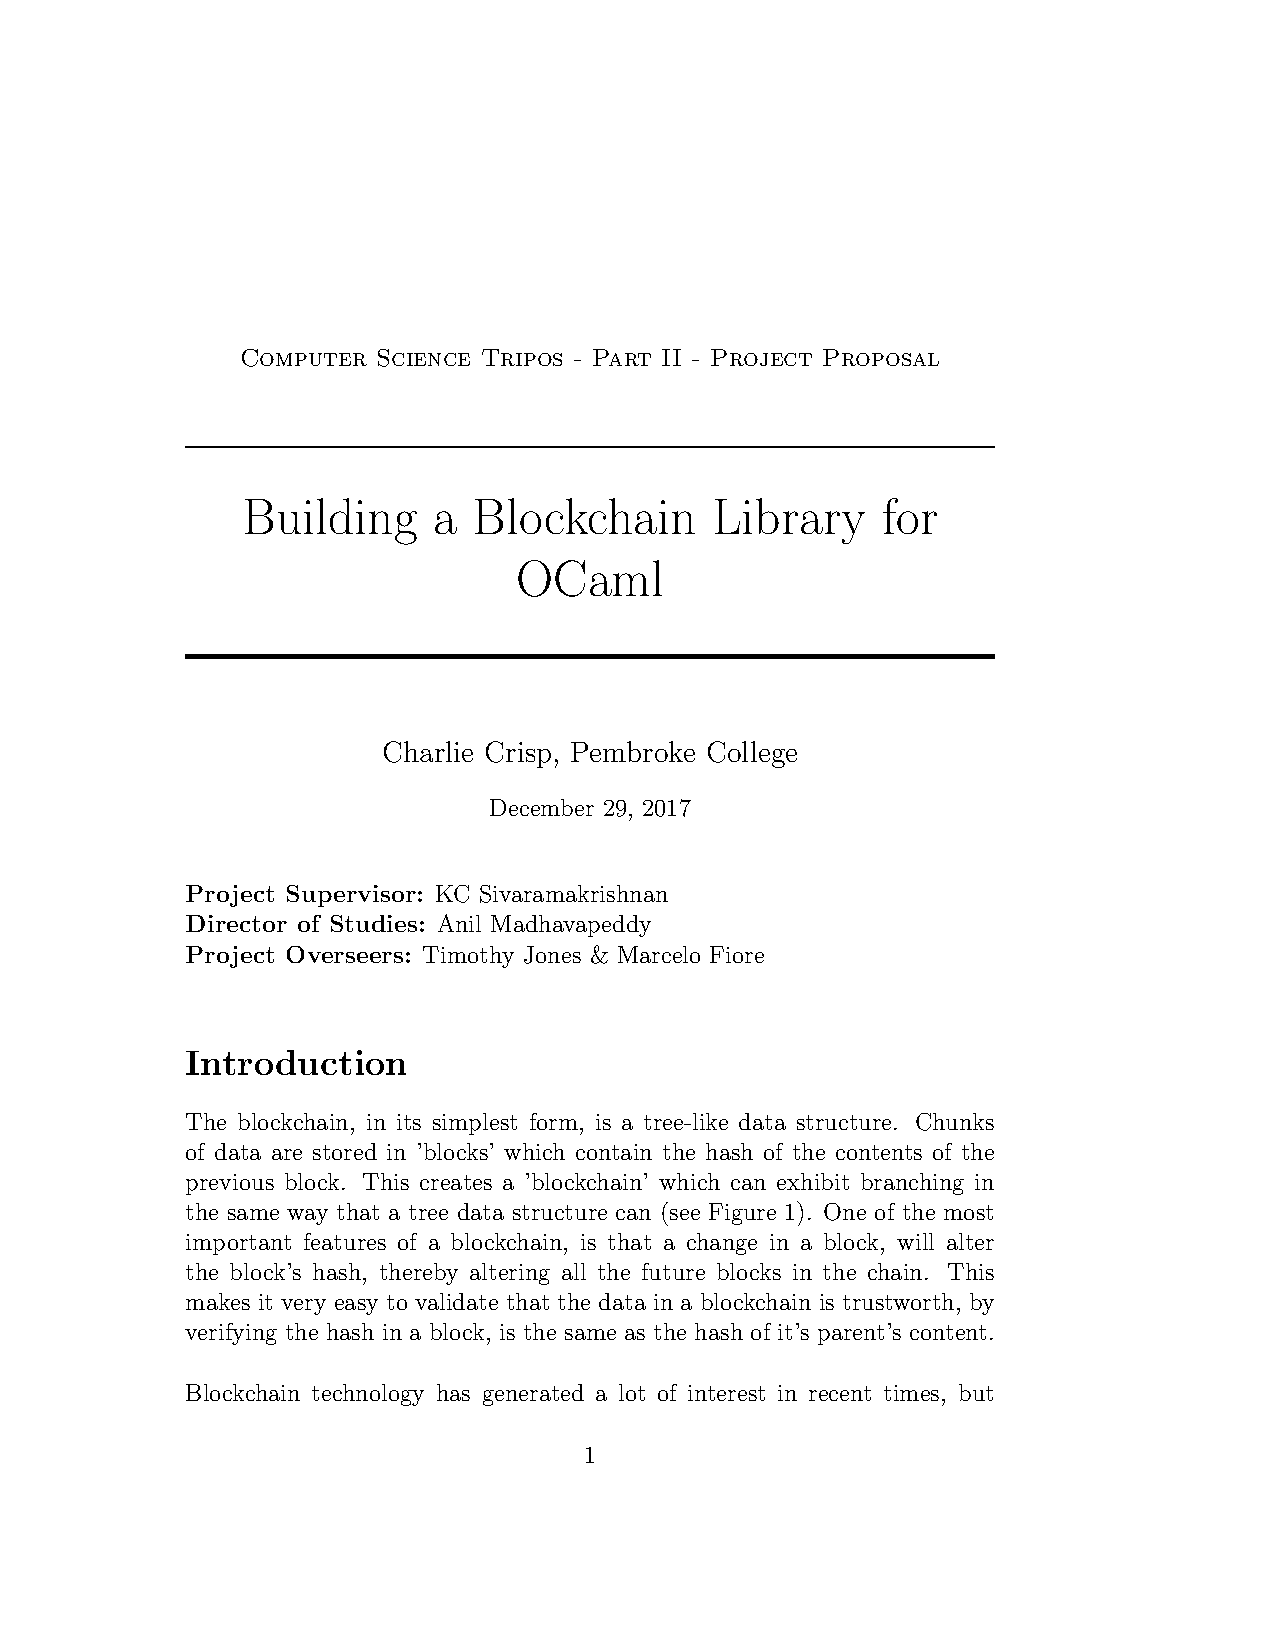
\includepdf[pages=-]{Part_II_Project_Proposal_Draft.pdf}
	
	\end{document}